%---------change this every homework
\def\yourid{Hyun Suk Ryoo}
\def\collabs{}
% -----------------------------------------------------
\def\duedate{9/13/18 12:30PM}
\def\duelocation{via Collab}
\def\prof{hr2ee}
\def\course{{Math 3100 (Introduction to Probability)}}%------
%-------------------------------------
%-------------------------------------

\documentclass[10pt]{report}
\usepackage[colorlinks,urlcolor=blue]{hyperref}
\usepackage[osf]{mathpazo}
\usepackage{amsmath,amsfonts,graphicx}
\usepackage{latexsym}
\usepackage[shortlabels]{enumitem}
\usepackage[top=1in,bottom=1.4in,left=1.5in,right=1.5in,centering]{geometry}
\usepackage{color}
\definecolor{mdb}{rgb}{0.3,0.02,0.02} 
\definecolor{cit}{rgb}{0.05,0.2,0.45} 
\pagestyle{myheadings}
\markboth{\yourid}{\yourid}
\usepackage{clrscode}
\usepackage{url}
\usepackage{qtree}
\usepackage{color}
\definecolor{mdb}{rgb}{0.3,0.02,0.02} 
\definecolor{cit}{rgb}{0.05,0.2,0.45} 
\pagestyle{myheadings}
\markboth{\yourid}{\yourid}
\usepackage{clrscode}
\usepackage{url}

\newenvironment{proof}{\par\noindent{\it Proof.}\hspace*{1em}}{$\Box$\bigskip}
\newcommand{\handout}{
   \renewcommand{\thepage}{}
   \noindent
   \begin{center}
      \vbox{
    \hbox to \columnwidth {\sc{\course} --- \prof \hfill}
    \vspace{-2mm}
    \hbox to \columnwidth {\sc due \MakeLowercase{\duedate} \duelocation \hfill {\LARGE\color{mdb}\yourid}}
      }
   \end{center}
      Homework \# 2
   \vspace*{2mm}
}
\newcommand{\solution}[1]{\medskip\noindent\textbf{Solution:}#1}
\newcommand{\bit}[1]{\{0,1\}^{ #1 }}
%\dontprintsemicolon
%\linesnumbered
\newtheorem{problem}{\sc\color{cit}section}
\newtheorem{practice}{\sc\color{cit}practice}
\newtheorem{lemma}{Lemma}
\newtheorem{definition}{Definition}

\def\therefore{\boldsymbol{\text{ }
\leavevmode
\lower0.4ex\hbox{$\cdot$}
\kern-.5em\raise0.7ex\hbox{$\cdot$}
\kern-0.6em\lower0.4ex\hbox{$\cdot$}
\thinspace\text{ }}}

\begin{document}
\thispagestyle{empty}
\handout
%----Begin your modifications here

\setcounter{chapter}{1}
\setcounter{section}{2}
\section{\sc\color{cit}Distributions}
\setcounter{subsection}{7}
\subsection{}

 \begin{enumerate}[(a)]
 \item $\mathbf{P(A \cup B) = 0.8} $ because of the proof shown...
 \begin{proof}
    \begin{align*}
    P(A \cup B) &= ? \\
    &= P(A) + P(B) - P(AB) \\
    &= 0.6 + 0.4 - 0.2 \\
    \therefore P(A \cup B) &= 0.8
    \end{align*}
\end{proof}
\item $\mathbf{P(A^c) = 0.4} $ because of the proof shown...
\begin{proof}
\begin{align*}
P(A^c) &= ? \\
&= 1 - P(A) \\
&= 1 - 0.6 \\
\therefore P(A^c) &= 0.4 \\
\end{align*}
\end{proof}
\item $\mathbf{P(B^c) =  0.6} $ because of the proof shown...
\begin{proof}
\begin{align*}
P(B^c) &= ? \\
&= 1 - P(B) \\
&= 1 - 0.4 \\
\therefore P(B^c) &= 0.6 \\
\end{align*}
\end{proof}
\item $\mathbf{P(A^cB) = 0.2} $ because of the proof shown...
\begin{proof}
The probability of intersection of $AB = 0.2$. This means that $0.2 $ probability is shared by $A$ and $B$. The question is asking for $P(A^cB) $. This is the space shared by $A^c $ and $B $. We can safely assume that $B \in A^c $. Therefore, $P(A^cB) = P(B) - P(AB) = 0.4 - 0.2 = 0.2 $
\end{proof}
\item $\mathbf{P(A \cup B^c) = 0.8} $ because of the proof shown...
\begin{proof}
\begin{align*}
P(A \cup B^c) &= ? \\
&= P(A) + P(B^c) - P(AB^c) \\
&= P(A) + 1 - P(B) - P(AB^c) \\
\end{align*}
$P(AB^c) = 0.4 $ due to the similar reasoning shown in part $(d) $. 
\begin{align*}
&= 0.6 + 1 - 0.4 - 0.4 \\
\therefore P(A \cup B^c) &= 0.8
\end{align*}
\end{proof}
\item $\mathbf{P(A^cB^c) = 0.2} $ due to the proof shown below. 
\begin{proof}
The only space that will be the intersection of $A^c $ and $B^c $ is space that is not in $A $ nor $B$. Therefore the space is for not A and not B. The space that is not shared with A or B in any way is $0.2$. 
\end{proof}
    \end{enumerate}
    \setcounter{subsection}{10}
\subsection{}
 \begin{enumerate}[(a)]
 \item 
 \begin{proof}\ \\
    \begin{align*}
    A \cup B \cup C &= (A \cup B) \cup C \\
    &= P(A \cup B) + P(C) - P((A \cup B) \cap C) \\
    &= P(A \cup B) + P(C) - P(A \cap C) \cup P(B \cap C) \\
    &= P(A \cup B) + P(C) - P(A \cap C) + P(B \cap C) - P(A \cap C \cap B \cap C) \\
    &= P(A \cup B) + P(C) - P(AC) + P(BC) - P(ABC) \\
    &= P(A) + P(B) - P(AB) + P(C) - (P(AC) + P(BC) - P(ABC)) \\
    &= P(A) + P(B) + P(C) - P(AB) - P(AC) - P(BC) + P(ABC) \\
    \end{align*}
    \end{proof}
\end{enumerate}
\section{\sc\color{cit}Conditional Probability and Independence}
\setcounter{subsection}{1}
 \subsection{}
This problem can be solved using conditional probability...
 \begin{proof}
 \begin{align*}
P(AB) &= P(A|B)P(B) \\
\textnormal{Where } A &=  \textnormal{ not defective} \\
\textnormal{Where } B &=  \textnormal{ made by city} B \\
&=(0.99)*(\frac{1}{3})\\
&= 0.33
 \end{align*}
 \end{proof} \\
 Therefore, the probability that the bulb is B and defective is $\mathbf{0.33} $ \\
 \subsection{}
Given that ...\\
 $A = $ rain today \\
 $P(A) = 0.4 $ \\
 $B = $ rain tomorrow \\
 $P(B) = 0.5 $ \\
 $P(AB) = 0.3 $ \\
 \begin{proof}
 \begin{align*}
 P(B|A) &= \frac{P(AB)}{P(A)} \\
 &= \frac{0.3}{0.4} \\
 &= 0.75
 \end{align*}
 \end{proof} \\
 Therefore, given it rains today the probability that it will rain tomorrow is $\mathbf{0.75}$
 \subsection{}
  \begin{enumerate}[(a)]
  \item Neither of the events occurs? \\
  \begin{align*}
  P(A) &= 0.1 \\
  P(B) &= 0.3 \\
  \end{align*}
   because they are independent events we can use the following equation \\
     \begin{align*}
  P(A^cB^c) &= P(A^c) * P(B^c) \\
  &= 0.9 * 0.7 \\
  &= 0.63 \\
  \end{align*}
  Therefore, neither of the events occurring is $\mathbf{0.63} $
\item At least one of the events occurs?
\begin{align*}
P(A \cup B) &= P(A) + P(B) - P(A)P(B) \\
&= 0.1 + 0.3 - 0.03 \\
&= 0.4 - 0.03 \\
&= 0.37 \\
\end{align*}
Therefore, the probability of at least one of the events happening is $\mathbf{0.37} $
\item exactly one of the events occurs? \\
This means the probability of $A $ happening with $B $ not happening or $B $ happening with $A $ not happening. \\
\begin{align*}
P(A^c \cap B) \cup P(A \cap B^c) &= ? \\
&= P(A^cB) + P(AB^c) \\
&= 0.9*0.3 + 0.1*0.7 \\
&= 0.34 \\
\end{align*}
Therefore, the probability of exactly one of the events occurring is $\mathbf{0.34} $
\end{enumerate}
\setcounter{subsection}{7}
 \subsection{}
$P(WW) = 0.3 $ = Both sides being white \\
$P(BW) = 0.5 $ = One side being white and one side being black \\
$P(BB) = 0.2 $ = Both sides being black \\
Assuming when placing the card both sides have an equally likely chance of being face up, we can show the following \\
\begin{center}
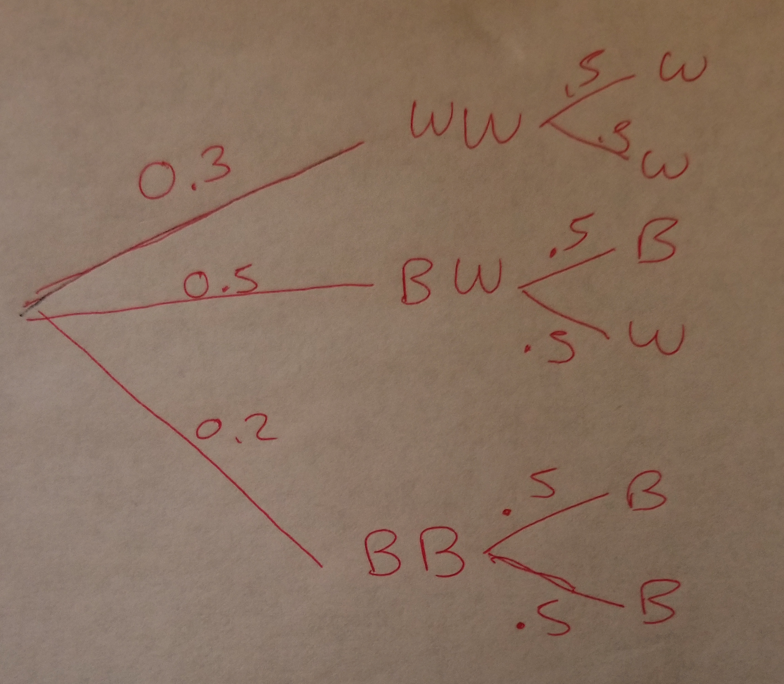
\includegraphics[scale=0.5]{diagram.png}
\end{center}
We should look at the probability of choosing a white card with the top side black is $0.5*0.5 $. \\
The probability that the top is black is $0.5*0.5 + 0.2*0.5 + 0.2*0.5 $ \\
The probability then is $\frac{0.25}{0.25 + 0.1 + 0.1} = \frac{0.25}{0.45} = \frac{5}{9}$ \\
Therefore, the probability of this occurring is $\mathbf{\frac{5}{9}} $
\section{\sc\color{cit}Special Problem (Bayes' Rule)}
\textbf{Problem} \\
A dashboard warning light is supposed to flash red if a car’s oil pressure is too low. On a certain model, the probability of the light flashing when it should is 0.99; 2\% of the time, though, it flashes for no apparent reason. If there is a 10\% chance that the oil pressure really is low, what is the probability that a driver needs to be concerned if the warning light goes on? \ \\
\ \\
\textbf{Solution} \\
Picture of work shown on the next page!!! Sorry for the inconvenience.\\\
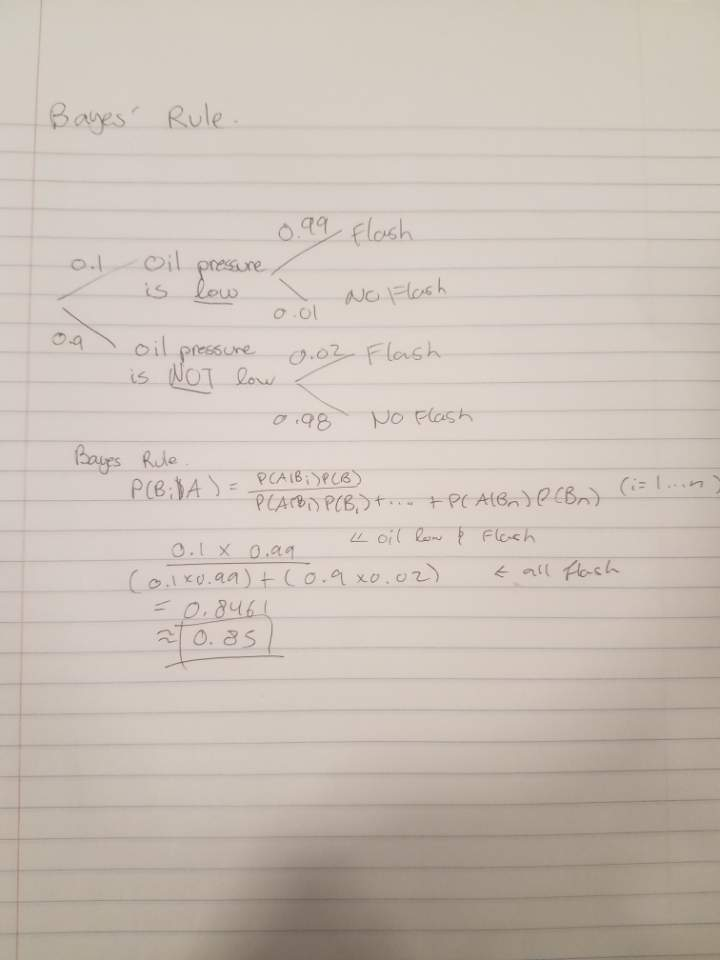
\includegraphics[scale=0.5]{bayes.jpeg}
\end{document}
